\documentclass{sigchi-ext}
% Please be sure that you have the dependencies (i.e., additional
% LaTeX packages) to compile this example.
\usepackage[T1]{fontenc}
\usepackage{textcomp}
\usepackage[scaled=.92]{helvet} % for proper fonts
\usepackage{graphicx} % for EPS use the graphics package instead
\usepackage{balance}  % for useful for balancing the last columns
\usepackage{booktabs} % for pretty table rules
\usepackage{ccicons}  % for Creative Commons citation icons
\usepackage{ragged2e} % for tighter hyphenation

% Some optional stuff you might like/need.
% \usepackage{marginnote} 
% \usepackage[shortlabels]{enumitem}
% \usepackage{paralist}
% \usepackage[utf8]{inputenc} % for a UTF8 editor only

%% EXAMPLE BEGIN -- HOW TO OVERRIDE THE DEFAULT COPYRIGHT STRIP --
% \copyrightinfo{Permission to make digital or hard copies of all or
% part of this work for personal or classroom use is granted without
% fee provided that copies are not made or distributed for profit or
% commercial advantage and that copies bear this notice and the full
% citation on the first page. Copyrights for components of this work
% owned by others than ACM must be honored. Abstracting with credit is
% permitted. To copy otherwise, or republish, to post on servers or to
% redistribute to lists, requires prior specific permission and/or a
% fee. Request permissions from permissions@acm.org.\\
% {\emph{CHI'14}}, April 26--May 1, 2014, Toronto, Canada. \\
% Copyright \copyright~2014 ACM ISBN/14/04...\$15.00. \\
% DOI string from ACM form confirmation}
%% EXAMPLE END

% Paper metadata (use plain text, for PDF inclusion and later
% re-using, if desired).  Use \emtpyauthor when submitting for review
% so you remain anonymous.
\def\plaintitle{Eine Vergleichsstudie: Java vs. Kotlin in Bezug auf Einstieger in der Android-App-Entwicklung}
\def\plainauthor{Franz Lea, Trummer Julia, Wieser Stefanie}
\def\emptyauthor{}
\def\plainkeywords{Java; Kotlin; Application Development; Android; Beginner;}
\def\plaingeneralterms{Documentation, Standardization}
\title{Eine Vergleichsstudie: Java vs. Kotlin in Bezug auf Einsteiger in der Android-App-Entwicklung}

\numberofauthors{6}
% Notice how author names are alternately typesetted to appear ordered
% in 2-column format; i.e., the first 4 autors on the first column and
% the other 4 auhors on the second column. Actually, it's up to you to
% strictly adhere to this author notation.
\author{%
  \alignauthor{%
    \textbf{Franz Lea}\\
    \affaddr{FH JOANNEUM Kapfenberg} \\
    \affaddr{Graz, Austria}\\
    \email{lea.franz@edu.fh-joanneum.at} }
  \alignauthor{%
    \textbf{Trummer Julia}\\
    \affaddr{FH JOANNEUM Kapfenberg} \\
    \affaddr{Graz, Austria}\\
    \email{julia.trummer@edu.fh-joanneum.at} }
  \alignauthor{%
    \textbf{Wieser Stefanie}\\
    \affaddr{FH JOANNEUM Kapfenberg} \\
    \affaddr{Graz, Austria}\\
    \email{stefanie.wieser2@edu.fh-joanneum.at} }
  }

% Make sure hyperref comes last of your loaded packages, to give it a
% fighting chance of not being over-written, since its job is to
% redefine many LaTeX commands.
\definecolor{linkColor}{RGB}{6,125,233}
\hypersetup{%
  pdftitle={\plaintitle},
%  pdfauthor={\plainauthor},
  pdfauthor={\emptyauthor},
  pdfkeywords={\plainkeywords},
  bookmarksnumbered,
  pdfstartview={FitH},
  colorlinks,
  citecolor=black,
  filecolor=black,
  linkcolor=black,
  urlcolor=linkColor,
  breaklinks=true,
}

% \reversemarginpar%

\begin{document}

%% For the camera ready, use the commands provided by the ACM in the Permission Release Form.
\CopyrightYear{2020}
\setcopyright{rightsretained}
\conferenceinfo{FH Joanneum}{April 19, 2020, Kapfenberg, AUSTRIA}
\isbn{978-1-4503-XXXX3/20/04}
\doi{https://doi.org/10.1145/3334480.XXXXXXX}
%% Then override the default copyright message with the \acmcopyright command.
\copyrightinfo{\acmcopyright}


\maketitle

% Uncomment to disable hyphenation (not recommended)
% https://twitter.com/anjirokhan/status/546046683331973120
\RaggedRight{} 

% Do not change the page size or page settings.
\begin{abstract}
  UPDATED---\today. This paper presents the results of a comparative study on Kotlin and Java as programming
  languages for realizing Android Applications. In particular we cover different fields like readability and coding costs. Furthermore, we undertook a closer look at the new features of Kotlin. Conclusively
  we will go over which coding language fits beginners best.
\end{abstract}

\keywords{\plainkeywords}



\section{Einleitung}
Derzeit werden immer mehr Android-Apps mit Kotlin entwickelt. Diese Programmiersprache ist im Gegensatz zu
Java relativ neu und wurde erstmals 2016 veröffentlicht. Zugleich ist Kotlin seit dem ersten Release als 
Open-Source-Software erhältlich und zielt im speziellen JVM (Java Virtual Machine) und Android ab. \cite{techyourchance}
In diesem Paper vergleichen wir Java mit Kotlin in den Aspekten Aufwand und Lesbarkeit. Darüber hinaus gehen wir auch
auf einige Sprachfeatures die Kotlin bietet ein. Zur Unterstützung unserer Vergleichsstudie
haben wir uns eine Slideshow-App ausgedacht und in beiden Programmiersprachen (Java und Kotlin) umgesetzt.
Ziel dieser Studie ist es herauszufinden, ob die Android Entwicklung in Java oder Kotlin
einfacher für Einsteiger ist.

\section{Kotlin}
Kotlin ist, gleich wie Java, eine objektorientierte Programmiersprache. Ein in dieser Sprache geschriebener Code kann 
in Bytecode für die JVM (Java Virtual Machine) kompiliert werden. Mit Kotlin können große Teile der 
Java-Boilerplate-Codes\footnote{Boilerplate-Code: Sind häufig verwendete und meist unveränderte Code-Snippets mit
gleicher Funktion.} verhindert werden.\cite{boilerplate}

\section{Java}
Java ist eine objektorientierte Programmiersprache und besteht aus den JDK (Java-Entwicklungstools) und der JRE
 (Java-Laufzeitumgebung). Grundsätzlich wird diese Programmiersprache für die Android Entwicklung 
 verwendet, weil sie sehr bekannt ist. TODO: Zitierung?


\begin{marginfigure}[-12pc]
  \begin{minipage}{\marginparwidth}
    \centering
    
\includegraphics[width=0.9\marginparwidth]{figures/kotlinlogo.png}
    \caption{JetBrains Kotlin Logo. Photo:
      \cczero~JetBrains s.r.o.}
  \end{minipage}
\end{marginfigure}

\begin{marginfigure}[1pc]
  \begin{minipage}{\marginparwidth}
    
\includegraphics[width=0.9\marginparwidth]{figures/javalogo.png}
    \caption{Java Technologies Java Logo
      \cczero~Java Technologies.}
  \end{minipage}
\end{marginfigure}


\section{Lesbarkeit}
Viele Entwickler meinen, dass Kotlin eine bessere Syntax als Java hat und deshalb besser
zu lesen ist. Nun ein Beispiel zu dieser Aussage: Wenn man versucht einen fremdsprachigen
Text zu lesen, ist es schwierig einen Satz zu verstehen ohne, dass man die Bedeutung der
einzelnen Wörter kennt. Versteht man aber mehrere Wörter und den Kontext, ist es einfacher den
Text zu lesen. Deshalb hat die Wahl der Sprache keinen Einfluss auf die Lesbarkeit, solange
der Kontext verständlich ist.
Was die Lesbarkeit betrifft, gibt es für Programmiersprachen keine objektiven Metriken.

\section{Sprachfeatures}
Kotlin bietet viele neue sprachenspezifische Features, die es von Java unterscheiden und Beginnern den Einstieg erleichtern. Im Folgenden wird auf vier solcher Features des Prototypes eingegangen.

\subsubsection{Null Sicherheit}
Die größten Fehlerquellen in Java-Systemen sind fehlende Null-Checks und die daraus entstehenden Null-Pointer Exceptions zur Laufzeit. In Kotlin können diese Fehler bereits zur Kompilierzeit aufgezeigt werden durch die klare Trennung von Referenzen, die Null sein können und Referenzen, die es nicht sein können. Variablen müssen dafür explizit als Nullable gekennzeichnet werden mit dem Anhängen eines Fragezeichens an den Datentyp bei der Variablendeklaration. Der Safe-Call-Operator (?.) kann dafür verwendet werden, dass immer entweder ein Ergebnis oder Null (ohne Null-Pointer Exception) zurückgegeben wird. \cite{moskala2017android} \\ \texttt{gpsText?.text = slide.GPS} \\ 

\subsubsection{Datenklassen}
Um Klassen als Datencontainer verwenden zu können, braucht es in Java min. einen Konstruktor und Getter/Setter. In Kotlin kann mit dem Keyword "data" eine Datenklasse erstellt werden, die ohne diesen Boilerplate-Code zurechtkommt. \\ \texttt{data class Slide(val id:Int,
                 var title:String = "untitled", ...)} \\ Der Compiler generiert hier Getter und Setter sowie die Methoden copy(), toString(), hashCode() und equals() automatisch im Hintergrund.
\cite{samuel2017programming} 

\subsubsection{Objekt Deklaration und Singletons}
In Kotlin gibt es das Sprachkonstrukt der Objekt Deklaration, mit dem das Singleton Pattern einfacher und kürzer als in Java implementiert werden kann. Dafür wird das Keyword "class" mit dem Keyword "object" ausgetauscht und somit kann nur mehr eine Instanz einer Klasse erstellt werden. \\\texttt{object Slideshow \{....\}} \\Einer Objekt Deklaration können Methoden und Properties genau wie einer Klasse hinzugefügt werden. \cite{moskala2017android} 


\subsubsection{Delegated Properties und Observer}
Auch mit diesem Sprachfeature gibt es eine Erleichterung bei der Verwendung eines Design Patterns im Gegensatz zu Java. Anstatt einer eigener Implementierung des Observer Patterns kann das in Kotlin integrierte Observable Delegate verwendet werden. Dabei ruft die Delegated Property eine Callback Funktion mit drei Parametern bei einer Änderung auf. \\ \texttt{private var currentSlideId: Int by \\Delegates.observable(0) \{ prop, oldSlideId, newSlideId -> .... \}} \\ Eine Delegated Property funktioniert prinzipiell wie eine reguläre Property, aber delegiert das Schreiben und Lesen von Werten an andere Funktionen. \cite{delegates}

\section{Lines of Code (LoC)}
Mittels dieser Metrik sollen die Umfänge der beiden Protoypen miteinander verglichen werden. Das Ziel ist es heraus zu finden welche der beiden Apps eine geringere Anzahl an Programmzeilen und Methoden hat.\footnote{Link zu den Apps: https://github.com/LeaFranz/KotlinJavaSlideshow} 

\begin{marginfigure}[-20pc]
  \begin{minipage}{\marginparwidth}
    \centering
    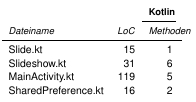
\includegraphics[width=1.05\marginparwidth]{figures/Kotlin-Tabelle.png}
    \caption{In dieser Tabelle sind alle wichtigen Files der in Kotlin implementierten Applikation samt Zeilenanzahl und Methodenanzahl enthalten.}
  \end{minipage}
\end{marginfigure}

\begin{marginfigure}[-3pc]
  \begin{minipage}{\marginparwidth}
    \centering
    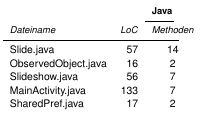
\includegraphics[width=1.05\marginparwidth]{figures/Java-Tabelle.png}
    \caption{In dieser Tabelle sind alle wichtigen Files der in Java implementierten Applikation samt Zeilenanzahl und Methodenanzahl enthalten. }
  \end{minipage}
\end{marginfigure}

\subsubsection{Vergleich}
Wie man deutlich an der Anzahl an Codezeilen sehen kann, hat der Java-Prototype um etwa ein Drittel mehr Zeilen als die in Kotlin implementierte Applikation. Des Weiteren ist deutlich zu erkennen, dass die Anzahl an Methoden in der in Java implementierten Applikation doppelt so hoch ist, wie in der Kotlin-App.
Dieser eindeutige Unterschied im Umfang entsteht unter anderem durch die in Kotlin integrierten Sprachfeatures. Einen wesentlichen Beitrag dazu leisten in Kotlin schnell zu implementierenden Patterns(Singleton, Observer) und die Verwendung einer Data Class, durch die auf Boilerplate-Code verzichtet werden kann.
Ein weiterer Unterschied liegt beim "Shuffle" einer ArrayList. Bei Kotlin gibt es bereits eine fertige, direkt verwendbare Methode. In der in Java implementierten Applikation braucht man dazu Collections und einen Comparator, wodurch der Code für die gleiche Funktionalität maßgeblich länger wird.

\section{Fazit}
Zusammenfassend kann man sagen, dass die in Kotlin implementierte Applikation nicht nur um ein Drittel des Codes kürzer, sondern auch durch die einzelnen Sprachfeatures deutlich einfacher zu implementieren ist.
Durch die Analyse der Prototypen anhand der verwendeten Metriken (Lesbarkeit, Sprachfeatures und Lines of Code) sind wir zu dem Schluss gekommen, dass wir Einsteigern für die Android-App-Entwicklung Kotlin empfehlen würden.

\balance{} 

\bibliographystyle{SIGCHI-Reference-Format}
\bibliography{sample}

\end{document}

%%% Local Variables:
%%% mode: latex
%%% TeX-master: t
%%% End:
